\documentclass[hidelinks]{ctexart}

\usepackage[sensei=潘海俊,gakka=電気力学,gakkabbr=ED,section=Housha]{styles/kurisu}

\usepackage{van-de-la-illinoise}
\usepackage{van-le-trompe-loeil}
\usepackage{stackengine}
\stackMath
\usepackage{scalerel}
\usepackage[outline]{contour}

\newlength\thisletterwidth
\newlength\gletterwidth
\newcommand{\leftrightharpoonup}[1]{%
{\ooalign{$\scriptstyle\leftharpoonup$\cr%\kern\dimexpr\thisletterwidth-\gletterwidth\relax
$\scriptstyle\rightharpoonup$\cr}}\relax%
}
\def\tensor#1{\settowidth\thisletterwidth{$\mathbf{#1}$}\settowidth\gletterwidth{$\mathbf{g}$}\stackon[-0.1ex]{\mathbf{#1}}{\boldsymbol{\leftrightharpoonup{#1}}}  }

\begin{document}

\section{电磁辐射} % (fold)
\label{sec:电磁辐射}

\subsection{规范势} % (fold)
\label{sub:规范势}

\subsubsection{源给定} % (fold)
\label{ssub:源给定}

\begin{cenum}
    \item 忽略场对源的影响,
    \item $-\partial_t \rho\pare{\+vr',t} = \grad'\+v\cdot \+vj\pare{\+vr',t}$,
    \item $t_r = t_r\pare{\+vr,t}$
    \[ -\+D{t_r}D{\rho\pare{\+vr,t_r}} = \brac{\div \+vj\pare{\+vr,t_r}}_{t_r}. \]
\end{cenum}

% subsubsection 源给定 (end)

\subsubsection{电磁场方程} % (fold)
\label{ssub:电磁场方程}

从Maxwell方程出发,
\[ \curl\pare{\curl \+vE} = \grad\pare{\div \+vE} - \laplacian \+vE = -\partial_t\pare{\curl \+vB} = -\mu_0 \partial_t \+vj - \rec{c^2}\partial_t^2 \+vE. \]
且
\[ \curl\pare{\curl \+vB} = \grad\pare{\div \+vB} - \laplacian \+vB = \mu_0 \curl \+vj + \rec{c^2}\partial_t \pare{\curl \+vE} = \mu_0 \curl \+vj - \rec{c^2}\partial_t \+vB. \]
从而
\[ \begin{cases}
    \displaystyle \Box{} \+vE = \rec{\epsilon_0} \pare{\grad \rho + \rec{c^2}\partial_t \+vj}, \\
    \displaystyle \Box{} \+vB = -\mu_0 \curl \+vj.
\end{cases} \]

% subsubsection 电磁场方程 (end)

\subsubsection{电磁势定义} % (fold)
\label{ssub:电磁势定义}

$\+vE = -\grad \varphi - \partial_t \+vA$, $\+vB = \curl \+vA$,
\begin{cenum}
    \item 规范变换$\varphi' = \varphi - \partial_t \psi$, $\+vA' = \+vA + \grad \psi$.
    \item Coulomb规范$\div \+vA = 0$.
    \item Lorentz规范$\displaystyle L = \div \+vA + \rec{c^2}\partial_{t} \varphi = 0$.
\end{cenum}

% subsubsection 电磁势定义 (end)

\subsubsection{势方程} % (fold)
\label{ssub:势方程}
在一般规范下,
    \[ \begin{cases}
        \Box{} \varphi + \partial_t L = \laplacian \varphi + \partial_t \pare{\div \+vA} = -\rho/\epsilon_0, \\
        \Box{} \+vA - \grad L = -\mu_0 \+vj.
    \end{cases} \]
\begin{cenum}
    \item Coulomb规范:
    \[ \begin{cases}
        \div \+vA = 0, \\
        \laplacian \varphi = -\rho/\epsilon_0,\\
        \Box{} \+vA = -\mu_0 \+vj_\perp,\quad \div \+vj_\perp = 0.
    \end{cases} \]
    \item Lorentz规范:
    \[ \begin{cases}
        \displaystyle L = \div \+vA + \rec{c^2}\partial_t \varphi = 0, \\
        \Box{}\varphi = -\rho/\epsilon_0, \\
        \Box{}\+vA = -\mu_0 \+vj.
    \end{cases} \]
\end{cenum}
\begin{ex}
    对于自由空间中的单色平面波,
    \[ \varphi\pare{\+vr,t} = \varphi_0 e^{i\pare{\+vk\cdot \+vr - \omega t}},\quad \+vA\pare{\+vr,t} = \+vA_0 e^{i\pare{\+vk\cdot \+vr - \omega t}}. \]
    Coulomb规范下, 三条方程分别给出
    \[ \varphi = 0,\quad \omega = kc,\quad \+vk\cdot \+vA = 0. \]
    此时
    \[ \+vE = -\partial_t \+vA = i\omega \+vA,\quad \+vB = \curl \+vA = i\+vk\times \+vA = \frac{\+vk\times \+vE}{\omega},\quad c\+vB = \+uk\times \+vE. \]
    Lorentz 规范下, 三条方程分别给出
    \[ \omega = kc,\quad \+vk\cdot \+vA = \frac{\omega}{c^2}\varphi \Rightarrow \varphi = c\+uk\cdot \+vA. \]
    此时
    \begin{align*}
        & \+vB = \curl \+vA = i\+vk\times \+vA,\\
        & \+vE = -\grad \varphi - \partial_t \+vA = -i\+vk\varphi + i\omega \+vA\\
        & = i\omega\brac{\+vA - \pare{\+uk\cdot \+vA}\+uk} = i\omega\+uk\times \pare{\+vA\times \+uk}\\
        &= c\+vB\times \+uk.
    \end{align*}
    令$\psi = \psi_0 e^{i\pare{\+vk\cdot \+vr - \omega t}}$, $\Box{}\psi = 0$. 令
    \[ \varphi' = \varphi - \partial_t\psi = \varphi + i\omega\psi = 0 \Rightarrow \psi_0 = \frac{i}{\omega}\varphi_0, \]
    故可以选择规范变换使$\varphi' = 0$.
\end{ex}

% subsubsection 势方程 (end)

% subsection 规范势 (end)

\subsection{推迟势} % (fold)
\label{sub:推迟势}

\subsubsection{局域电荷电流分布的推迟势} % (fold)
\label{ssub:推迟势}

对于局域电荷, 电流分布, 有
\[ \resumath{\begin{cases}
    \displaystyle \varphi\pare{\+vr,t} = \rec{4\pi\epsilon_0} \iiint \rd{V'}\, \frac{\rho\pare{\+vr',t_r}}{\+gr}, \\
    \displaystyle \+vA\pare{\+vr,t} = \frac{\mu_0}{4\pi} \iiint \rd{V'}\, \frac{\+vj\pare{\+vr',t_r}}{\+gr}.
\end{cases}} \]
\begin{cenum}
    \item 推迟时间$\displaystyle t_r = t - \frac{\+gr}{c} = t_r\pare{\abs{\+vr-\+vr'},t}$, 故
    \[ \+gr = c\pare{t-t_r} = c\Delta t > 0. \]
    \item 其物理含义为,
    \begin{cenum}
        \item 不同位置的源对场的贡献由不同时刻的分布决定.
        \begin{center}
            \begin{tikzpicture}
                \draw (0,0) -- (2,0) -- (2,-0.5) -- (0,-0.5) -- (0,0);
                \draw[latex-latex] (0,-0.7) -- (2,-0.7) node[midway,below] {$\Delta L$};
                \draw (2,0) node[above left](tr1) {$t_{r1}$};
                \draw[-latex] (2,-0.25) -- (3,-0.25) node[right] {$\+vv$};
                \draw[-latex] (tr1.east) -- (tr1-|4,0);
                \draw (-3,0) -- (-1,0) -- (-1,-0.5) -- (-3,-0.5) -- (-3,0);
                \draw (-3,0.5) node[above left](tr2) {$t_{r2}$};
                \draw[-latex] (tr2.east) -- (tr2-|4,0);
                \draw (4,0) node[below] {$P,t$} -- (4,1);
                \draw[latex-latex] (-3,-1.5) -- (2,-1.5) node[midway,below] {$\Delta L'$};
            \end{tikzpicture}
        \end{center}
        \item 可以将积分区域限定为源不为零的区域. 设实验室参考系下场源的长为$\Delta L$, 以$\+vv$运动,
        \begin{cenum}
            \item 在$t_{r1}$时刻, 细棒右端发出的信号恰好到达$P$点, 其余各点到达$P$的信号源一定在$t_{r1}$之后.
            \item $t_{r1}$时刻后, 细棒右端的信号不可能再到达此时的$P$点.
            \item $t_{r2}$时刻, 细棒左端发出的信号恰好到达$P$点, 其余各点到达$P$的信号源一定在$t_{r2}$之前.
            \item $t_{r2}$之前, 细棒右端的信号不可能到达此时的$P$点.
            \item $\displaystyle \Delta L' - \Delta L = v\pare{t_{r1} - t_{r2}} = \frac{v}{c}\Delta L'$, 从而
            \[ \Delta L' = \frac{\Delta L}{1-\beta},\quad \beta = \frac{v}{c}. \]
        \end{cenum}
        \begin{center}
            \begin{tikzpicture}
                \draw (0,0) -- (2,0) -- (2,-0.5) -- (0,-0.5) -- (0,0);
                \draw (-3,0) -- (-1,0) -- (-1,-0.5) -- (-3,-0.5) -- (-3,0);
                \draw[-latex] (2,-0.25) -- (3,-0.25) node[right] {$\+vv$};
                \draw[latex-latex] (0,0.2) -- (2,0.2) node[midway,above] {$\Delta L$};
                \draw[latex-latex] (-3,0.7) -- (2,0.7) node[midway,above] {$\Delta L'$};
                \draw (2,0) node[above right](tr1) {$t_{r1}$};
                \draw (-3,0) node[above left](tr2) {$t_{r2}$};
                \draw[-latex] (2,-0.5) -- (3,-1.5);
                \draw[-latex] (-3,-0.5) -- (-1,-2.5);
                \draw (3,-1.5) -- (-1,-2.5) node[midway,below] {$P,t$};
            \end{tikzpicture}
        \end{center}
        对于一般的方向,
        \[ \Delta L' - \Delta L = v\pare{t_{r1} - t_{r2}} = \frac{v}{c}\Delta L'\cos\theta = \pare{\+v\beta\cdot \+u{\+gr}}\Delta L', \]
        从而
        \[ \Delta L' = \frac{\Delta L}{1-\+v\beta\cdot \+u{\+gr}} \Rightarrow \Delta V' = \frac{\Delta V}{1-\+v\beta\cdot \+u{\+gr}}. \]
    \end{cenum}
    \item 上述结论可推广至一般区域.
\end{cenum}
\begin{figure}[ht]
    \centering
    \incfig{6cm}{SpacetimeDiagram}
    \caption{Minkowski时空图下的表观长度}
\end{figure}

% subsubsection 推迟势 (end)

\subsubsection{证明} % (fold)
\label{ssub:证明}

\begin{cenum}
    \item 如下基本关系成立,
    \[ \grad \+gr = \+u{\+gr},\quad \grad\rec{\+gr} = -\frac{\+u{\+gr}}{\+gr^2},\quad \div \frac{\+u{\+gr}}{\+gr^2} = 4\pi\delta\pare{\+v{\+gr}},\quad \div \frac{\+u{\+gr}}{\+gr} = \rec{\+gr^2}. \]
    最后一条关系可通过
    \[ \div \frac{\+u{r}}{r} = \div \frac{\+vr}{r^2} = \frac{\div \+vr}{r^2} + \pare{\grad \rec{r^2}}\cdot \+vr = \frac{3}{r^2} - \frac{2\+ur}{r^3}\cdot \+vr = \rec{r^2}. \]
    注意到
    \[ \int_{r\le a}\rd{V}\, \div \frac{\+ur}{r} = \oint_{r=a}\rd{\+v\sigma}\cdot \frac{\+ur}{r} = a\oint_{r=a}\rd{\Omega} = 4\pi a. \]
    而
    \[ \int_{r\le a}\rd{V}\, \rec{r^2} = 4\pi a \]
    同样成立, 故上式适用于原点处而不会出现$\delta$函数项. 同时成立
    \[ t_r = t - \frac{\+gr}{c} \Rightarrow \partial_t t_r = 1,\quad \grad t_r = -\frac{\+u{\+gr}}{c}. \]
    对于一般的函数,
    \[ f=f\pare{\+vr',t_r} \Rightarrow \+DtDf = \+D{t_r}Df,\quad \grad f = \pare{\grad t_r} \+D{t_r}Df = -\frac{\+u{\+gr}}{c}\dot{f}. \]
    其中$\dot f$在推迟时刻计算.
    \item d'Alembert方程$\displaystyle \laplacian \varphi - \rec{c^2}\partial_t^2 \varphi = -\rho/\epsilon_0$,
    \begin{align*}
        & \grad \frac{\rho\pare{\+vr,t_r}}{\+gr} = \rho\pare{\grad \rec{\+gr}} + \rec{\+gr}\grad \rho = -\frac{\rho \+u{\+gr}}{\+gr^2} - \frac{\dot{\rho}\+u{\+gr}}{c\+gr}. \\
        & \laplacian \frac{\rho}{\+gr} = \div \grad \frac{\rho}{\+gr} = -\brac{\rho\div \frac{\+u{\+gr}}{\+gr^2} + \frac{\+u{\+gr}}{\+gr^2}\cdot \grad \rho} - \rec{c}\brac{\dot \rho \div \frac{\+u{\+gr}}{\+gr} + \frac{\+u{\+gr}}{\+gr}\cdot \grad \dot\rho} \\
        &= -\brac{\rho\cdot 4\pi\delta\pare{\+v{\+gr}} - \frac{\dot\rho}{c\+gr^2}} - \rec{c}\brac{\frac{\dot\rho}{\+gr^2} - \frac{\ddot\rho}{c\+gr}}. \\
        & \Rightarrow \laplacian \frac{\rho}{\+gr} = -4\pi\rho\pare{\+vr',t_r}\delta\pare{\+v{\+gr}} + \frac{\ddot{\rho}}{c^2\+gr},\quad \rec{c^2}\partial_t^2 \frac{\rho}{\+gr} = \frac{\ddot\rho}{c^2\+gr}.\\
        & \Rightarrow \laplacian \varphi - \rec{c^2}\partial_t^2\varphi = \rec{4\pi\epsilon_0}\int \rd{V'}\,\pare{\laplacian - \rec{c^2}\partial_t^2} \frac{\rho}{\+gr} \\
        &= -\rec{\epsilon_0} \int \rd{V'}\, \rho\pare{\+vr,t_r}\delta\pare{\+v{\+gr}} \\
        &= -\rec{\epsilon_0} \rho\pare{\+vr,t}.
    \end{align*}
    \item Lorentz规范$\displaystyle L = \div \+vA + \rec{c^2}\partial_t \varphi = 0$.
    \begin{align*}
        \div \+vA &= \frac{\mu_0}{4\pi} \iiint \rd{V'}\, \div \frac{\+vj\pare{\+vr',t_r}}{\+gr} \\
        &= \frac{\mu_0}{4\pi} \iiint \rd{V'}\, \brac{-\grad'\+v\cdot \frac{\+vj\pare{\+vr',t_r}}{\+gr} + \frac{\brac{\grad'\+v\cdot \+vj\pare{\+vr',t_r}}_{t_r}}{\+gr}} \\
        &= \rec{4\pi\epsilon_0 c^2}\curb{-\oint \rd{\+v\sigma'}\cdot \frac{\+vj}{\+gr} - \int \rd{V'}\, \frac{\partial_t \rho\pare{\+vr',t_r}}{\+gr} } \\
        &= -\rec{c^2} \partial_t \varphi.
    \end{align*}
    如果将$t_r = t-\+gr/c$修改为$t_a = t+\+gr/c$, 上述结论仍然成立, 仅仅由于其不科学而排除之.
\end{cenum}

% subsubsection 证明 (end)

\subsubsection{电磁场} % (fold)
\label{ssub:电磁场}
Jefimenko(神野\ 冨美子, 1966), Schott(1912)得到
\begin{align*}
    \+vE &= -\grad\varphi - \partial_t \+vA \Rightarrow \resumath{\+vE = \rec{4\pi\epsilon_0}\int \rd{V'}\, \brac{\frac{\rho \+u{\+gr}}{\+gr^2} + \frac{\dot{\rho}\+u{\+gr}}{c\+gr} - \frac{\dot{\+vj}}{c^2\+gr} }.} \\
    \+vB &= \curl \+vA = \frac{\mu_0}{4\pi} \int \rd{V'}\, \curl \frac{\+vj\pare{\+vr',t_r}}{\+gr} \\
    &= \frac{\mu_0}{4\pi} \int \rd{V'}\,\brac{\pare{\grad \rec{\+gr}} \times \+vj + \rec{\+gr}\curl \+vj} \\
    &= \frac{\mu_0}{4\pi} \int \rd{V'}\,\brac{-\frac{\+u{\+gr}}{\+gr^2}\times \+vj - \frac{\+u{\+gr}}{c\+gr}\times \+vj}. \\
    \Rightarrow & \resumath{\+vB = \frac{\mu_0}{4\pi} \int \rd{V'}\,\brac{\frac{\+vj}{\+gr^2}\times \+u{\+gr} + \frac{\dot{\+vj}}{c\+gr}\times \+u{\+gr}}.}
\end{align*}
可知辐射场按$1/\+gr$衰减.

\begin{sample}
    \begin{ex}
        设$\+v\kappa = \+v\kappa_0\pare{t}\Theta\pare{t}$, 其生成电磁场如何.
    \end{ex}
    \begin{solution}
        显然$\varphi = 0$, 注意到$\+gr\,\rd{\+gr} = z\,\rd{z}$,
        \begin{align*}
            \+vA\pare{z,t} &= \frac{\mu_0}{4\pi} \int_0^{2\pi} \int_0^\infty s\,\rd{s}\, \frac{\+v\kappa\pare{t-\+gr/c}}{\+gr} \\
            &= \frac{\mu_0}{2} \int_{\abs{z}}^{ct} \rd{\+gr}\, \+v\kappa\pare{t - \frac{\+gr}{c}} \\
            &= \frac{\mu_0 c}{2}\int_0^{t-\abs{z}/c} \rd{\xi}\,\+v\kappa\pare{\xi}. \\
            \+vE &= -\partial_t \+vA = -\frac{\mu_0 c}{2}\+v\kappa\pare{t-\frac{\abs{z}}{c}}. \\
            \+vB &= \curl \+vA = \pare{\grad z} \times \+DzD{\+vA}\\ &= \+uz\times \brac{-\rec{c} \frac{\mu_0 c}{2} \+dzd{\abs{z}}\+v\kappa\pare{t-\frac{\abs{z}}{c}}} = \frac{\sgn z}{c}\+uz\times \+vE. \qedhere
        \end{align*}
    \end{solution}
\end{sample}
\begin{sample}
    \begin{ex}
        设$I = I\pare{t}\Theta\pare{t}$, 其生成电磁场如何.
    \end{ex}
    \begin{solution}
        显然$\varphi = 0$, $\displaystyle \+vA\pare{s,t} = \+uz \frac{\mu_0}{4\pi} \int_{-\infty}^{+\infty} \rd{z}\, \frac{I_0\pare{t-\+gr/c}\Theta\pare{t-\+gr/c}}{\+gr}$. 当$t<s/c$, 必定有$\+vA = 0$. 否则
        \begin{align*}
            \+vA\pare{s,t} &= \+uz \frac{\mu_0}{2\pi} \int_0^{\sqrt{c^2t^2 - s^2}} \rd{z}\, \frac{I_0\pare{t-\+gr/c}}{\+gr}, \\
            I_0\pare{t} &= I_0, \\
            \+vA\pare{s,t} &= \+uz \frac{\mu_0I_0}{2\pi} \int_0^{\sqrt{c^2t^2 - z^2}} \frac{\rd{z}}{\sqrt{z^2+s^2}} \\
            &= \+uz \frac{\mu_0 I_0}{2\pi}\ln \frac{ct + \sqrt{c^2t^2 - s^2}}{s}.
        \end{align*}
        电磁场可自行求解. 如果$I_0 = kt$如何?
    \end{solution}
\end{sample}
\begin{sample}
    \begin{ex}
        设原点处有理想电偶极子$\+vp\pare{t}$, 其$\rho\pare{\+vr,t}$和$\+vj\pare{\+vr,t}$如何, $\varphi$, $\+vA$如何, $\+vS$如何.
    \end{ex}
    \begin{solution}
        静止于原点处的
        \begin{align*}
            \varphi\pare{\+vr,t} &= \frac{\+vp\cdot \+vr}{4\pi\epsilon_0 r^3} = -\rec{4\pi\epsilon_0} \+vp\cdot \grad \rec{r}\\
            \Rightarrow \rho &= -\epsilon_0 \laplacian \varphi = \rec{4\pi} \+vp\cdot \grad\pare{-4\pi \delta\pare{\+vr}} \\
            \Rightarrow \rho\pare{\+vr,t} &= -\+vp\pare{t}\cdot \grad \delta\pare{\+vr} \\
            \Rightarrow -\partial_t \rho\pare{\+vr,t} &= +\div\brac{\dot{\+vp}\pare{t}\delta\pare{\+vr}} = \div \+vj\pare{\+vr,t} \\
            \Rightarrow \+vj\pare{\+vr,t} &= \dot{\+vp}\pare{t}\delta\pare{\+vr}. \\
            \+vA\pare{\+vr,t} &= \frac{\mu_0 }{4\pi}\int \rd{V'} \frac{\dot{\+vp}\pare{t-\+gr/c}\delta\pare{\+vr'}}{\+gr} = \frac{\mu_0 \dot{\+vp}_r}{4\pi r},\quad \+vp_r = \+vp\pare{t-\frac{r}{c}}. \\
            L &= \div \+vA + \rec{c^2}\partial_t \varphi = 0, \\
            \Rightarrow \partial_t \varphi &= -c^2 \div \+vA = -\rec{4\pi\epsilon_0} \div \frac{\dot{\+vp}_r}{r}, \\
            \div \frac{\dot{\+vp}_r}{r} &= \pare{\grad \rec{r}}\cdot \dot{\+vp}_r + \rec{r}\div \dot{\+vp}_r \\
            &= -\frac{\+ur\cdot \dot{\+vp}_r}{r^2} - \frac{\+ur\cdot \ddot{\+vp}_r}{cr}. \\
            \+vA &= \frac{\mu_0 \dot{\+vp}_r}{4\pi r}, \\
            \varphi &= \rec{4\pi\epsilon_0} \brac{\frac{\+vp_r\cdot \+ur}{r^2} + \frac{\dot{\+vp}_r \cdot \+ur}{cr}}. \\
            \+vB &= \curl \+vA = \frac{\mu_0}{4\pi} \curl \frac{\dot{\+vp}_r}{r} = \boxed{\frac{\mu_0}{4\pi}\brac{\frac{\dot{\+vp}_r}{r^2} + \frac{\ddot{\+vp}_r}{cr}}\times \+ur.} \\
            \grad \frac{\+ur}{r^{n-1}} &= -\frac{n\+ur\+ur - \tensor{I}}{r^n}. \\
            \+vE &= -\grad\varphi - \partial_t \+vA = -\rec{4\pi\epsilon_0}\begin{cases}
                \displaystyle \pare{\grad \frac{\+ur}{r^2}}\cdot \+vp_r + \pare{\grad \+vp_r} \cdot \frac{\+ur}{r^2} \\[.5em] \displaystyle + \rec{c}\pare{\grad \frac{\+ur}{r}}\cdot\dot{\+vp}_r + \pare{\grad \dot{\+vp}_r}\cdot \frac{\+ur}{cr} + \frac{\ddot{\+vp}_r}{c^2 r}
            \end{cases}\\
            &= \rec{4\pi\epsilon_0}\begin{cases}
                \displaystyle \frac{3\pare{\+vp_r\cdot \+ur}\+ur - \+vp_r}{r^3} + \frac{\pare{\dot{\+vp}_r \cdot \+ur}\+ur}{c^2} + \frac{2\pare{\dot{\+vp}_r\cdot \+ur}\+ur - \dot{\+vp}_r}{cr^2} \\[.5em]
                \displaystyle + \frac{\pare{\ddot{\+vp}_r \cdot \+ur}\+ur}{c^2 r} - \frac{\ddot{\+vp}_r}{c^2 r}
            \end{cases} \\
            &= \boxed{\rec{4\pi\epsilon_0}\brac{\frac{3\pare{\+vp_r \cdot \+ur}\+ur - \+vp_r}{r^3} + \frac{3\pare{\dot{\+vp}_r \cdot \+ur}\+ur - \dot{\+vp}_r}{cr^2} + \frac{\pare{\ddot{\+vp}_r\cdot \+ur}\+ur - \ddot{\+vp}_r}{c^2r}}.}
        \end{align*}
        设$\+vp$有变化特征时间$\tau$, 则
        \[ \dot{\+vp}_r \approx \frac{\+vp_r}{\tau},\quad \ddot{\+vp}_r \approx \frac{\+vp_r}{\tau^2}. \]
        从而
        \begin{align*}
            \+vB & \approx \frac{\mu_0}{4\pi} \curb{\frac{p_r}{r^2\cdot \tau}, \frac{p_r}{r\cdot c\tau^2}}, \\
            \+vE & \approx \rec{4\pi\epsilon_0} \curb{\frac{p_r}{r^3}, \frac{p_r}{r^2 \cdot c\tau}, \frac{p_r}{r\cdot c^2 \tau^2}}.
        \end{align*}
        在近区, $r \ll c\tau$,
        \[ E \approx \rec{r^3},\quad B \approx \rec{r^2},\quad \frac{E}{cB} \sim \frac{\tau}{\epsilon_0 \mu_0 cr} = \frac{c\tau}{r} \gg 1. \]
        在中间区, $r \approx c\tau$, 所有项的贡献量级相同. 在远区$r\gg c\tau$,
        \[ E \approx \rec{r},\quad B \approx \rec{r}. \qedhere \]
    \end{solution}
\end{sample}
对于$\+vp = p\pare{t}\+uz$, 上述偶极辐射的Poynting矢量满足
\begin{align*}
    \+ur\cdot \+vS &= \rec{\mu_0} \+ur\cdot{\+vE\times \+vB} = \rec{\mu_0}\pare{\+ur\times \+vE}\cdot \+vB, \\
    \frac{\+vB}{\mu_0} &= \rec{4\pi}\brac{\frac{\dot{\+vp}_r}{r} + \frac{\ddot{\+vp}_r}{c}}\frac{\sin \theta}{r} \+u\phi, \\
    \+ur\times \+vE &= \rec{4\pi\epsilon_0}\brac{\frac{p_r}{r^2} + \frac{\dot{p}_r}{cr} + \frac{\ddot{p}_r}{c^2}}\frac{\sin\theta}{r}\+u\phi, \\
    \+ur \cdot \+vS &= \rec{4\pi}\rec{4\pi\epsilon_0}\brac{\frac{p_r \dot{p}_r}{r^3} + \frac{p_r \ddot{p}_r + \dot{p}_r^2}{cr^2} + \frac{2\dot{p}_r\ddot{p}_r}{c^2 r} + \frac{\ddot{p}_r^2}{c^3}} \frac{\sin^2\theta}{r^2}. \\
    \int \rd{\Omega}\,\sin^2\theta &= \int_0^{2\pi}\int_{-1}^1 \pare{1-\cos\theta^2}\,\rd{\cos\theta} = \frac{8\pi}{3}. \\
    \oint_{r=R}\rd{\+v\sigma}\cdot \+vS &= \frac{2}{3}\rec{4\pi\epsilon_0} \brac{\+dtd{}\pare{\frac{p_r^2}{2r^3} + \frac{p_r\dot{p}_r}{cr^2} + \frac{\dot{p}_r^2}{c^2r} } + \frac{\ddot{p}_r^2}{c^3} }.
\end{align*}
全导数由近区贡献, 对时间平均后消失. 真正向外的能流为最后一项.

% subsubsection 电磁场 (end)

% subsection 推迟势 (end)

\subsection{谐振电流及其辐射场} % (fold)
\label{ssub:谐振电流及其辐射场}

\subsubsection{Poynting矢量} % (fold)
\label{ssub:poynting矢量}

单位时间内从$\rd{\+v\sigma}$流出的能量为
\[ \rd{\+v\sigma}\cdot \+vS = \pare{\+ur\cdot \+vS}r^2\,\rd{\Omega}. \]
辐射功率的角分布
\[ \+d{\Omega}d{P} = \lim_{r\rightarrow \infty} \pare{\+ur\cdot \+vS}r^2 = \frac{r^2}{\mu_0}\+ur\cdot \pare{\+vE\+_rad_\times \+vB\+_rad_}. \]
而Poynting定理表明
\[ -\+vE\cdot \+vj = \partial_t w + \div \+vS \Rightarrow -\int_V \rd{V}\, \+vE\cdot \+vj = \+dtdW + \oint_{\partial V}\rd{\+v\sigma}\cdot \+vS. \]
对于$V$为全空间, 且电流为谐振电流的情形,
\[ \expc{P} = -\half \Re \int \rd{V}\, \+vE^*\cdot \+vj. \]

% subsubsection poynting矢量 (end)

\subsubsection{谐振电流及其电磁势} % (fold)
\label{ssub:谐振电流及其电磁势}

对于
\[ \+vj\pare{\+vr,t} = \+vj_0\pare{\+vr}e^{-i\omega t},\quad \partial_t = -i\omega, \]
\begin{cenum}
    \item 电荷
    \[ \rho\pare{\+vr,t} = \rho_0\pare{\+vr}e^{-i\omega t} = \frac{i}{\omega}\div \+vj\pare{\+vr,t}, \]
    而
    \[ \div \+vj = -\partial_t \rho = +i\omega \rho. \]
    \item 矢势
    \begin{align*}
        \+vA\pare{\+vr,t} &= \+vA_0\pare{\+vr}e^{-i\omega t} = \frac{\mu_0}{4\pi}\int \rd{V'}\, \frac{\+vj\pare{\+vr',t}}{\+gr}e^{ik\+gr}, \\
        \varphi\pare{\+vr,t} &= \rec{4\pi\epsilon_0} \int \rd{V'}\, \frac{\rho\pare{\+vr',t}}{\+gr} e^{ik\+gr} = \pare{-\frac{ic^2}{\omega}} \frac{\mu_0}{4\pi} \int \rd{V'}\, \frac{\div \+vj\pare{\+vr',t}}{\+gr} e^{ik\+gr} \\
        &= -i\frac{c^2}{\omega}\div \+vA\pare{\+vr,t}.
    \end{align*}
    也可以直接通过Lorentz规范
    \[ 0 = \div \+vA + \rec{c^2}\partial_t \varphi = \div \+vA - i\frac{\omega}{c^2}\varphi \]
    可得相同的结论.
    \item 磁场$\+vB = \curl \+vA$.
    \item 电场$\+vE = \displaystyle i \frac{c^2}{\omega} \curl \+vB$在源外成立.
    \item 定义源尺度$R = V^{1/3}$, 场源距离$R$, 波长$\displaystyle \lambda = \frac{2\pi}{\lambda}$, 约化波长$\tilde{\lambda} = 1/k$.
\end{cenum}

% subsubsection 谐振电流及其电磁势 (end)

\subsubsection{场划分} % (fold)
\label{ssub:场划分}

\begin{cenum}
    \item 小场源近似: $R \ll \+gr,\pare{r'\ll r}$, 且$R \ll \lambda$, 即$kr'\ll 1$.
    \item 场区划分:
    \[ \begin{cases}
        \text{近场区:} & R\ll \lambda,\quad k\+gr\ll 1,\\
        \text{感应区:} & R\approx \lambda,\quad k\+gr\approx 1, \\
        \text{辐射区:} & R \gg \lambda,\quad k\+gr \gg 1.
    \end{cases} \]
\end{cenum}

% subsubsection 场划分 (end)

\subsubsection{辐射场} % (fold)
\label{ssub:辐射场}

\paragraph{近似1} % (fold)
\label{par:近似1}

设$R\ll \+gr$, 即$r' \ll r$,
\[ \+vA\pare{\+vr,t} \approx \frac{\mu_0}{4\pi r}\int \rd{V'}\, \+vj\pare{\+vr',t} e^{ik\+gr}. \]
注意到
\begin{align*}
    k\+gr &= k\pare{\+vr - \+vr'} = ke^{-\+vr'\cdot \grad}r = k\pare{1 - \+vr'\cdot \grad + \rec{2!}\+vr'\+vr':\grad\grad + \cdot }r \\
    &= k\brac{r - \+vr'\cdot \+ur + \half \+vr'\+vr':\frac{\tensor{I} - \+ur\+ur}{r} + \cdots} \\
    &= kr - kr'\pare{\+ur\cdot \+ur'} + \half kr'\frac{r'}{r}\brac{1 - \pare{\+ur\cdot\+ur'}^2} + \cdots.
\end{align*}
故相因子上的$k\+gr$不可近似.

% paragraph 近似1 (end)

\paragraph{近似2} % (fold)
\label{par:近似2}

$R\lessapprox \lambda$, 即$kr' \lessapprox 1 \Rightarrow k\+gr \approx \+vk\cdot \+v{\+gr}$, 其中$\displaystyle \+vk = \frac{\omega}{c}\+ur$. 此时相因子上的$k\+gr$可使用远场近似.
\begin{align*}
    \+vA\pare{\+vr,t} &= \frac{\mu_0 e^{ikr}}{4\pi r}\int \rd{V'}\, \+vj\pare{\+vr',t} e^{-i\+vk\cdot \+vr'} \\
    &= \frac{\mu_0 e^{i\pare{kr - \omega t}}}{4\pi r}\int \rd{V'}\, \+vj_0\pare{\+vr'} e^{-i\+vk\cdot \+vr'}.
\end{align*}
相应的
\begin{align*}
    \grad e^{-i\+vk\cdot \+vr'} &= -ik\pare{\grad \+ur}\cdot \+vr' e^{-i\+vk\cdot \+vr'} \\
    &= -ik\frac{\tensor{I} - \+ur\+ur}{r}\cdot \+vr' e^{-i\+vk\cdot \+vr'}, \\
    \grad \frac{e^{ikr}e^{-i\+vk\cdot \+vr'}}{r} &= \pare{\grad \rec{r}} e^{ikr} e^{-i\+vk\cdot \+vr'} + \frac{e^{-i\+vk\cdot \+vr'}}{r}\grad e^{ikr} + \frac{e^{ikr}}{r}\grad e^{-\+vk\cdot \+vr'} \\
    &\approx O\pare{\rec{r^2}} + O\pare{\frac{k}{r}} + O\pare{\frac{kr'}{r^2}}.
\end{align*}

% paragraph 近似2 (end)

\paragraph{近似3} % (fold)
\label{par:近似3}

$\lambda \ll r$, $\pare{kr \gg 1}$, 从而第一项和第三项可忽略. $\grad \leftarrow i\+vk$,
\[ \frac{e^{-i\+vk\cdot \+vr'}}{r}\grad e^{ikr} = \frac{e^{-i\+vk\cdot \+vr'}}{r}i\+vk e^{ikr}. \]

% paragraph 近似3 (end)

\paragraph{总结} % (fold)
\label{par:总结}

在近似$R\lessapprox \lambda \ll r$下, 对于谐振电流
\begin{cenum}
    \item $\displaystyle \+vA\pare{\+vr,t} = \frac{\mu_0 e^{ikr}}{4\pi r}\int \rd{V'}\, \+vj\pare{\+vr',t} e^{-i \+vk\cdot \+vr'}$.
    \item $\displaystyle \partial_t \leftrightarrow -i\omega$, $\displaystyle \grad \leftrightarrow i\+vk = i\frac{\omega}{c}\+ur \leftrightarrow -\frac{\+ur}{c}\partial_t$.
    \item $\displaystyle \+vB = i\+vk\times \+vA = \rec{c}\dot{\+vA}\times \+ur$, $\displaystyle i\+vk\times \+vB = -\frac{i\omega}{c^2}\+vE$, 从而
    \[ \resumath{\begin{cases}
        \displaystyle \+vB = i\+vk\times \+vA = \rec{c}\dot{\+vA}\times \+ur,\\
        \displaystyle \+vE = c\+vB\times \+ur.
    \end{cases}} \]
\end{cenum}
因此辐射场是TEM球面波, $\pare{\+vE,\+vB,\+vk}$构成右手正交系, $E = cB$.

% paragraph 总结 (end)

% subsubsection 辐射场 (end)

\subsubsection{辐射功率} % (fold)
\label{ssub:辐射功率}
\vspace{-\baselineskip}
\begin{align*}
    \expc{\+vS} &= \expc{\rec{\mu_0} \+vE\times \+vB} = \rec{2\mu_0}\Re\pare{\+vE^* \times \+vB}, \\
    \Rightarrow \expc{\+vS} &= \frac{c}{2\mu_0}\abs{\+vB}^2 \+ur,\quad \abs{\+vB}^2 = \+vB^*\cdot \+vB, \\
    \+d\Omega d{\expc{P}} &= \abs{\expc{S}}r^2 = \frac{c}{2\mu_0}\abs{\+vB}^2 r^2, \\
    \expc{P} &= \oint \rd{\Omega}\,\+d\Omega d{\expc{P}}.
\end{align*}
\[ \resumath{\+d\Omega d{\expc{P}} = \frac{c}{2\mu_0}\abs{\+vB}^2 r^2.} \]

% subsubsection 辐射功率 (end)

% subsection 谐振电流及其辐射场 (end)

\subsection{小场源辐射} % (fold)
\label{sub:小场源辐射}

此时$R\ll \lambda$, $R\ll r$, $\lambda \ll r$, 即$R\ll\lambda \ll r$.

\subsubsection{局域电流} % (fold)
\label{ssub:局域电流}

考察$\+vj = \+vj\pare{\+vr',t}$, $\rho = \rho\pare{\+vr',t}$,
\begin{align*}
    \grad'\+v\cdot \+vj &= -\partial_t \rho, \\
    \grad'\+v\cdot\pare{\+vj\+vr'} &= -\pare{\partial_t \rho}\+vr' + \+vj, \\
    \grad'\+v\cdot\pare{\+vj\+vr'\+vr'} &= -\pare{\partial_t \rho} \+vr'\+vr' + \+vj\+vr' + \+vr'\+vj, \\
    \int \rd{V'}\, \+vj\pare{\+vr',t} &= \dot{\+vp}\pare{t}, \\
    \int \rd{V'}\, \+vj\+vr' &= \half \int \rd{V'}\, \pare{\+vj \+vr' + \+vr' \+vj} + \half \rd{V'}\,\pare{\+vj\+vr' - \+vr'\+vj} \\
    &= \+vm\pare{\+vr}\times \tensor{I} + \rec{6}\dot{\tensor{D}}\pare{t} + \rec{6}\dot{g}\tensor{I}.
\end{align*}
其中
\begin{align*}
    \+vp\pare{t} &= \int \rd{V'}\, \+vr'\rho\pare{\+vr',t}, \\
    \+vm\pare{t} &= \half \int \rd{V'}\, \+vr'\times \+vj\pare{\+vr',t}, \\
    \tensor{D}\pare{t} &= \int \rd{V'}\,\rho\pare{\+vr',t}\pare{3\+vr'\+vr' - r'^2 \tensor{I}}, \\
    g\pare{t} &= \int \rd{V'}\, \rho\pare{\+vr',t}r'^2.
\end{align*}

% subsubsection 局域电流 (end)

\subsubsection{磁矢势展开} % (fold)
\label{ssub:磁矢势展开}

$kr' \ll 1 \Rightarrow e^{-i\+vk\cdot \+vr'} \approx 1-i\+vk\cdot \+vr'$,
\begin{align*}
    \+vA\pare{\+vr,t} &\approx \frac{\mu_0 e^{ikr}}{4\pi r}\brac{\int \rd{V'}\, \+vj\pare{\+vr',t} - i\int \rd{V'}\, \+vj\pare{\+vr',t} \+vr'\cdot \+vk} \\
    &= \frac{\mu_0 e^{ikr}}{4\pi r}\brac{\dot{\+vp}\pare{t} - i\+vm\pare{t}\times \+vk - \frac{i}{6}\dot{\tensor{D}}\cdot \+vk - \frac{i}{6}\dot{g}\+vk} \\
    &= \frac{\mu_0 e^{ikr}}{4\pi r}\brac{\+vp + \rec{c}\dot{\+vm}\times \+ur + \rec{6c}\+ur\cdot \ddot{\tensor{D}} + \rec{6c}\ddot{g}\+ur} \\
    &= \frac{\mu_0}{4\pi r}\brac{\dot{\+vp}_r + \rec{c}\dot{\+vm}_r \times \+ur + \rec{6c}\+ur\cdot \ddot{\tensor{D}}_r + \rec{6c}\ddot{g}_r \+ur}.
\end{align*}
其中
\[ \+vp_r = \+vp\pare{t - \frac{r}{c}} = \+vp_0 e^{-i\omega\pare{t-r/c}} = \+vp_0 e^{-i\omega t}e^{ikr}. \]
令$\displaystyle \+vA' = \+vA + \grad \psi = \+vA + i\+vk\psi = \+vA - \frac{\+ur}{c}\dot{\psi}$,
\[ \frac{\dot{\psi}}{c} = \frac{\mu_0 e^{ikr}}{4\pi r}\cdot \frac{\ddot{g}}{6c} \Leftarrow \psi = \frac{\mu_0 e^{ikr}}{24\pi r} \dot{g},\quad \Box{} \psi =  0. \]

% subsubsection 磁矢势展开 (end)

\subsubsection{电偶极辐射} % (fold)
\label{ssub:电偶极辐射}

$\displaystyle \+vA\pare{\+vr,t} = \frac{\mu_0 e^{ikr}}{4\pi r}\dot{\+vp}\pare{t}$,
\begin{cenum}
    \item 场
    \begin{resume}
        \vspace{-\baselineskip}
        \begin{align*}
            \+vB &= \rec{c}\dot{\+vA}\times \+ur = \frac{\mu_0 e^{ikr}}{4\pi cr} \ddot{\+vp}\times \+ur, \\
            \+vE &= c\+vB\times \+ur = \frac{\mu_0 e^{-ikr}}{4\pi r}\pare{\ddot{\+vp}\times \+ur}\times \+ur.
        \end{align*}
    \end{resume}
    \item 辐射功率
    \begin{align*}
        \+d\Omega d{\expc{P}} &= \frac{c}{2\mu_0} \abs{\+vB}^2 r^2 = \frac{\mu_0}{32\pi^2 c} \abs{\ddot{\+vp}\times \+ur}^2, \\
        \expc{P} &= \frac{\abs{\ddot{\+vp}}^2}{12\pi\epsilon_0 c^3} \propto \omega^4.
    \end{align*}
    \[ \resumath{\+d\Omega d{\expc{P}} = \frac{\mu_0}{32\pi^2 c} \abs{\ddot{\+vp}\times \+ur}^2,\quad \expc{P}\frac{\abs{\ddot{\+vp}}^2}{12\pi\epsilon_0 c^3} \propto \omega^4.} \]
    \item 关于电偶极矩:
    \begin{align*}
        \+vp &= \+vp_0 e^{-i\omega t} = \pare{\+vp\+_R_ + i\+vp\+_I_} e^{-i\omega t}, \\
        \Re \+vp &= \+vp\+_R_ \cos \omega t + \+vp\+_I_\sin \omega t. \\
        \expc{P} &= \rec{32\pi \epsilon_0 c^3} \int \rd{\omega}\, \pare{\ddot{\+vp}^*\times \+ur}\cdot \pare{\ddot{\+vp}\times \+ur} \\
        &= \rec{32\pi^2 \epsilon_0 c^3} \int \rd{\Omega}\, \brac{\abs{\ddot{\+vp}}^2 - \abs{\ddot{\+vp}\cdot \+ur}^2}. \\
        \+ur &= \alpha_i \+ux_i,\quad \alpha_1 = \sin\theta\cos\phi,\quad \alpha_2 = \sin\theta \sin\phi,\quad \alpha_3 = \cos\theta, \\
        \abs{\ddot{\+vp}\cdot \+ur}^2 &= \pare{\ddot{p}_i^* \alpha_i}\pare{\ddot{p}_j \alpha_j},\quad \int \rd{\Omega}\, \alpha_i \alpha_j = \frac{4\pi}{3}\delta_{ij}, \\
        \int \rd{\Omega}\, \abs{\ddot{\+vp}}^2 &= \abs{\ddot{\+vp}}^2 \cdot 4\pi, \\
        \int \rd{\Omega}\, \abs{\ddot{\+vp}\cdot \+ur}^2 &= \int \rd{\Omega}\, \ddot{p}_i^* \ddot{p}_j \alpha_i \alpha_j = \ddot{p}_i^* \ddot{p}_j\cdot \frac{4\pi}{3}\delta_{ij} = \abs{\ddot{\+vp}}^2 \cdot \frac{4\pi}{3} \\
        &\Rightarrow \expc{P} = \frac{\abs{\ddot{\+vp}}^2}{12\pi\epsilon_0 c^3} \propto \omega^4.
    \end{align*}
\end{cenum}

\begin{sample}
    \begin{ex}
        定向电偶极子, $\+vp\pare{t} = \+vp_0 e^{-i\omega t}$,
        \begin{align*}
            \+vB &= -\frac{\omega^2 \mu_0 p_0}{4\pi c}\frac{\sin\theta e^{i\psi}}{r}\+u\phi, \quad \psi = kr- \omega t, \\
            \+vE &= c\+vB\times \+ur = -\frac{\omega^2 \mu_0 p_0}{4\pi} \frac{\sin \theta e^{i\psi}}{r}\+u\theta.
        \end{align*}
        \begin{cenum}
            \item 电场沿经向, 磁场沿纬向.
            \item $\displaystyle \+d\Omega d{\expc{P}} \propto \omega^4 \sin^2\theta \Rightarrow \begin{cases}
                \theta = 0, & \text{辐射强}, \\
                \theta = 0,\pi, & \text{无辐射}.
            \end{cases}$ 对于固定的$p_0$, $P\propto \omega^4$.
            \item $\displaystyle \dot{\+vp}\pare{t} = \int \rd{V'} \, \+vj\pare{\+vr',t} \sim I\+_m_e^{-i\omega t}$.
        \end{cenum}
    \end{ex}
\end{sample}
\begin{sample}
    \begin{ex}
        短天线
        \[ I\pare{z,t} = I\+_m_\pare{1-2\frac{\abs{z}}{l}}e^{-i\omega t},\quad \abs{z} \le \frac{l}{2}. \]
        相应的
        \begin{align*}
            \dot{\+vp}\pare{t} &= \+uz \int_{-l/2}^{l/2} I\pare{z,t} \,\rd{z} = 2\+uz I\+_m_ e^{-i\omega t}\int_0^{l/2} \pare{1-2\frac{z}{l}}\,\rd{z} \\
            &= \half I\+_m_ l e^{-i\omega t}\+uz = -i\omega \+vp. \\
            \ddot{\+vp} &= -\omega^2 \+vp = -i\half I\+_m_\frac{\omega l}{2\pi cl/\lambda} e^{-i\omega t} = -i\pi c\frac{l}{\lambda}I\+_m_e^{-i\omega t}. \\
            \expc{P} &= \frac{\pi}{12\epsilon_0 c}\pare{\frac{l}{\lambda}}^2 I\+_m_^2 = \half I\+_m_^2 R_r.
        \end{align*}
        其中$R_r$谓辐射电阻,
        \[ R_r = \frac{\pi}{6}\sqrt{\frac{\mu_0}{\epsilon_0}}\pare{\frac{l}{\lambda}}^2 = \SI{197}{\ohm}\pare{\frac{l}{\lambda}}^2. \]
        \begin{cenum}
            \item $\displaystyle \expc{P} \propto \omega^2$.
            \item $R_r$表示天线的辐射能力.
            \item 对于短天线, $R_r \sim \SI{1}{\ohm}$.
        \end{cenum}
    \end{ex}
\end{sample}

\begin{sample}
    \begin{ex}
        对于匀速圆周运动的点电荷,
        \[ R \ll \lambda \sim \rec{R} = \frac{c}{\omega} \Rightarrow v = \omega R \ll c. \]
        \begin{cenum}
            \item 电偶极矩
            \begin{align*}
                & \Re \+vp = eR\pare{\+ux \cos\omega t + \+uy \sin\omega t} \\
                & \Rightarrow \+vp = eR\pare{\+ux + i\+uy} e^{-i\omega t} \\
                & \Rightarrow {\+vp} = eR\pare{\+ur\sin\theta + \+u\theta\cos\theta + i\+u\phi} e^{i\pare{\phi - \omega t}}, \\
                & \Rightarrow \ddot{\+vp} = -e\omega^2 R\pare{\+ur\sin\theta + \+u\theta\cos\theta + i\+u\phi} e^{i\pare{\phi - \omega t}}.
            \end{align*}
            \item 辐射场
            \begin{align*}
                \+vB &= \frac{\mu_0 e^{ikr}}{4\pi c r}\ddot{\+vp}\times \+ur = \frac{ea}{4\pi\epsilon_0 c^3} \frac{-i\+u\theta + \+u\phi\cos\theta}{r}e^{i\psi}, \\
                \+vE &= c\+vB\times\+ur = \frac{ea}{4\pi\epsilon_0 c^2} \frac{\+u\theta\cos\theta + i\+u\phi}{r}e^{i\psi}, \\
                \psi &= kr - \omega t + \phi.
            \end{align*}
            偏振度
            \[ \tilde{R} = \frac{E_\phi}{E_\theta} = \frac{i}{\cos\theta}, \]
            从而
            \[ \begin{cases}
                \theta = 0, & \mathrm{RCP}, \\
                \theta = \pi, & \mathrm{LCP},
            \end{cases}\quad \begin{cases}
                0<\theta<\pi/2, & \text{右椭},\\
                \pi/2 < \theta<\pi, & \text{左椭},
            \end{cases}\quad \theta = \pi/2,\quad \text{线偏}. \]
            \item 辐射功率
            \begin{align*}
                & \+d\Omega d{\expc{P}} = \frac{c}{2\mu_0} \abs{\+vB}^2 r^2 = \frac{e^2a^2}{32\pi^2 \epsilon_0 c^3}\pare{1+\cos^2\theta}, \\
                & \expc{P} = \frac{e^2 a^2}{6\pi\epsilon_0 c^3} = \frac{2}{3}\frac{e_s^2 a^2}{c^3},\quad e_s^2 = \frac{e^2}{4\pi\epsilon_0} = \SI{1.44}{\mega\eV\cdot \femto\meter}.
            \end{align*}
        \end{cenum}
    \end{ex}
\end{sample}
\paragraph{磁偶极子辐射} % (fold)
\label{par:磁偶极子辐射}

\begin{align*}
                \+vA &= \frac{\mu_0 e}{4\pi cr} \dot{\+vm}\times \+ur, \\
                \+vB &= \rec{c} \dot{\+vA}\times \+ur = \frac{\mu_0 r^{ikr}}{4\pi c^2 r} \pare{\ddot{\+vm}\times \+ur}\times \+ur, \\
                \+vE &= c\+vB\times \+ur, \\
                \+d\Omega d{\expc{P}} &= \frac{c}{2\mu_0}\abs{\+vB}r^2 = \frac{\mu_0}{32\pi^2c^3} \abs{\ddot{\+vm}\times\+ur}^2, \\
                \Rightarrow \expc{P} &= \frac{\abs{\ddot{\+vm}}^2}{12\pi \epsilon_0 c^5}.
\end{align*}
\begin{resume}
磁偶极子辐射
    \begin{flalign*}
        & && \+vB = \rec{c} \dot{\+vA}\times \+ur = \frac{\mu_0 r^{ikr}}{4\pi c^2 r} \pare{\ddot{\+vm}\times \+ur}\times \+ur, && \+vE = c\+vB\times \+ur, && \\
        & && \+d\Omega d{\expc{P}} = \frac{\mu_0}{32\pi^2c^3} \abs{\ddot{\+vm}\times\+ur}^2, && \expc{P} = \frac{\abs{\ddot{\+vm}}^2}{12\pi \epsilon_0 c^5}. &&
    \end{flalign*}
\end{resume}

% paragraph 磁偶极子辐射 (end)
            
\begin{sample}
    \begin{ex}
        圆电流$I\pare{t} = I\+_m_ e^{-i\omega t}$.
        \begin{align*}
            \+vm &= \pi R^2 I\+_m_ e^{-i\omega t}\+uz, \\
            \ddot{\+vm} &= -\pi \pare{\omega R}^2 I\+_m_ e^{-i\omega t}\+uz = -4\pi^3 c^2 \pare{\frac{R}{\lambda}}^2 I\+_m_ e^{-i\omega t}\+uz, \\
            \+d{\omega}d{\expc{P}} &= \half \pi^4 \mu_0 c \pare{\frac{R}{\lambda}}^4 I\+_m_^2 \sin^2\theta \propto \sin^2\theta. \\
            \expc{P} &= \frac{4\pi^5}{3}\mu_0 c\pare{\frac{R}{\lambda}}^4 I\+_m_^4 = \half I\+_m_^2 R_r.
        \end{align*}
        辐射电阻
        \[ R_r = \frac{8\pi^5}{3}\sqrt{\frac{\mu_0}{\epsilon_0}}\pare{\frac{R}{\lambda}}^4. \]
        \begin{cenum}
            \item $\expc{P}\propto \omega^4$, $I\+_m_$一定.
            \item $\displaystyle \frac{\pare{R_r}\+_M_}{\pare{R_r}\+_P_} \xlongequal{R=l} = 16\pi^4 \pare{\frac{R}{\lambda}}^2 = \pare{4\pi^2 \frac{R}{l}}^2 \approx \pare{40\frac{R}{\lambda}}^2$.
            \begin{cenum}
                \item $\displaystyle \frac{R}{\lambda} > \rec{40}$, 磁偶极辐射占优.
                \item $f = \SI{50}{\mega\hertz}$, $\lambda = \SI{6}{\meter}$, $R = \SI{15}{\centi\meter}$, 磁偶极辐射占优.
                \item $f = \SI{200}{\mega\hertz}$, $\lambda = \SI{1.5}{\meter}$, $R = \SI{15}{\centi\meter}$, 磁偶极辐射占大优.
            \end{cenum}
        \end{cenum}
    \end{ex}
\end{sample}

% subsubsection 电偶极辐射 (end)

\subsubsection{电四极辐射} % (fold)
\label{ssub:电四极辐射}

\vspace{-\baselineskip}
\begin{align*}
    \+vA &= \frac{\mu_0 e^{ikr}}{24\pi cr} \+ur\cdot \ddot{\tensor{D}}, \\
    \+vB &= \frac{\mu_0 e^{ikr}}{24\pi c^2 r} \+ur \cdot \dddot{\tensor{D}} \times \+ur, \\
    \+d\Omega d{\expc{P}} &= \frac{\mu_0}{1152\pi^2 c^3}\abs{\+ur\cdot \dddot{\tensor{D}}\times \+ur}^2 \\
    \Rightarrow \expc{P} &= \frac{\abs{\dddot{\tensor{D}}}^2}{1440\pi \epsilon_0 c^3}.
\end{align*}
\begin{sample}
    \begin{ex}
        对于如下图所示的系统,
        \begin{center}
            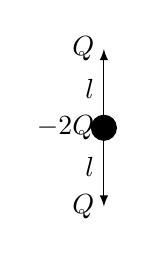
\begin{tikzpicture}
                \draw[latex-] (0,-1) -- (0,0) node[midway,left] {$l$};
                \draw (0,-1) node[left] {$Q$};
                \draw (0,0) node[circle, fill] {};
                \draw (0,0) node[left] {$-2Q$};
                \draw[-latex] (0,0) -- (0,1) node[midway,left] {$l$};
                \draw (0,1) node[left] {$Q$};
            \end{tikzpicture}
        \end{center}
        \vspace{-\baselineskip}
        \begin{align*}
            & Q\pare{t} = Q_0 e^{-i\omega t} \Rightarrow I = \+dtdQ = -i\omega Q_0 e^{-i\omega t} = -iI\+_m_e^{-i\omega t}. \\
            & D_1 = D_2 = -\half D_3, \\
            & \tensor{D} = -\half D_3 \pare{\+ux\+ux + \+uy\+uy} + D_3 \+uz\+uz = \half D_3 \pare{3\+uz\+uz - \tensor{I}}, \\
            & D_3 = \sum q\pare{3z^2 - z^2} = 2\sum qz^2 = 4Ql^2. \\
            & \dddot{D}_3 = 4Ql^2\pare{-i\omega}^3 = 4i\omega Q_0 \pare{\omega l}^2 \\
            & \Rightarrow \dddot{D}_3 = 4i I\+_m_ \pare{\frac{2\pi c}{\lambda}l}^2 e^{-i\omega t} = 16i\pi^2 c^2\pare{\frac{l}{\lambda}}^2 I\+_m_ e^{-i\omega t}. \\
            & \abs{\+ur\cdot \dddot{\tensor{D}}\times \+ur}^2 = \abs{\half \dddot{D}_3 \+ur\cdot\pare{3\+uz\+uz - \tensor{I}}\times \+ur}^2 = \frac{9}{4}\abs{\dddot{D}_3}^2 \sin^2\theta\cos^2\theta. \\
            \Rightarrow \+d\Omega d{\expc{P}} &= \half \pi^2 \mu_0 c \pare{\frac{l}{\lambda}}^4 I\+_m_^2 \sin^2\theta \cos^2\theta.
        \end{align*}
        当$\theta = \pi/4$或$\theta = 3\pi/4$有最强辐射, 而$\theta = 0$, $\theta = \pi/2$和$\theta=\pi$处无辐射.
        \[ \Rightarrow \expc{P} = \half I\+_m_^2 R_r,\quad R_r = \frac{8\pi^3}{15}\sqrt{\frac{\mu_0}{\epsilon_0}}\pare{\frac{l}{\lambda}}^4. \]
    \end{ex}
\end{sample}

% subsubsection 电四极辐射 (end)

% subsection 小场源辐射 (end)

\subsection{天线辐射} % (fold)
\label{sub:天线辐射}

形如下图的天线谓中心馈电型天线,
\begin{center}
    \begin{tikzpicture}
        \draw
        (-2,-1) to[sinusoidal voltage source] (-2,1) -- (-1,1) -- (-1,0.25) to[short,i=\mbox{}] (0,0.25) -- (0,2) (-2,-1) -- (-1,-1) -- (-1,-0.25) to[short,i<=\mbox{}] (0,-0.25) -- (0,-2) (0,2) node[left] {$l/2$} (0,-2) node[left] {$-l/2$};
    \end{tikzpicture}
\end{center}
\subsubsection{天线电流} % (fold)
\label{ssub:天线电流}

$\displaystyle I\pare{z,t} = I_0 \sin k\pare{\frac{l}{2} - \abs{z}}e^{-i\omega t}$, $\displaystyle \abs{z} \le \frac{l}{2}$.
\begin{cenum}
    \item $m = l/\lambda$ $\displaystyle \Rightarrow m=\frac{kl}{2\pi}$,
    \[ \Rightarrow I\pare{z,t} = I_0 \sin \pare{m\pi - k\abs{z}},\quad k\abs{z} \le m\pi. \]
    \item $\displaystyle m = \half$者谓半波天线,
    \[ \Rightarrow I\pare{z,t} = I_0 \cos kz,\quad \abs{z} \le \frac{\lambda}{4}. \]
    \item 峰值电流$I\+_m_$,
    \[ \begin{cases}
        m \ge 1/2 \Rightarrow I\+_m_ = I_0, \\
        m < 1/2 \Rightarrow I\+_m_ = I_0 \sin m\pi, \\
        m \ll 1/2 \Rightarrow I\+_m_ \approx I_0 m\pi.
    \end{cases} \]
\end{cenum}

% subsubsection 天线电流 (end)

\subsubsection{矢量势} % (fold)
\label{ssub:矢量势}

\vspace{-\baselineskip}
\begin{align*}
    \+vA\pare{\+vr,t} &= \frac{\mu_0 e^{i\pare{kr - \omega t}}}{4\pi r}\int \rd{V'}\, \+vj_0\pare{\+vr'} e^{-i\+vk\cdot \+vr'} \\
    &= \+uz \frac{\mu_0 e^{i\psi}}{4\pi r}\int_{-l/2}^{l/2} \rd{z'}\, I_0 \sin\pare{m\pi - k\abs{z'}} e^{-ikz'\cos\theta} \\
    &= \+uz \frac{\mu_0 I\+_0_ e^{i\psi}}{4\pi kr} \int_0^{m\pi} \rd{\rho}\, {2\sin\pare{m\pi - \xi}\cos \pare{\xi \cos\theta}} \\
    &= \+uz \frac{\mu_0 I_0 e^{i\psi}}{4\pi kr} \curb{\frac{\cos \brac{m\pi - \pare{1-\cos\theta}\xi}}{1-\cos\theta} + \frac{\cos\brac{m\pi - \pare{1+\cos\theta}\xi}}{1+\cos\theta}}_0^{m\pi} \\
    &= \+uz \frac{\mu_0 I_0 e^{i\psi}}{4\pi kr}\pare{\rec{1-\cos\theta} + \rec{1+\cos\theta}}\brac{\cos\pare{m\pi \cos\theta} - \cos \pare{m\pi}} \\
    &= \+uz \frac{\mu_0 I_0 e^{i\psi}}{2\pi kr} \frac{g\pare{\theta}}{\sin\theta}.
\end{align*}
其中
\[ g\pare{\theta} = \frac{\cos \pare{m\pi \cos\theta} - \cos m\pi}{\sin\theta}. \]

% subsubsection 矢量势 (end)

\subsubsection{辐射场} % (fold)
\label{ssub:辐射场}

\vspace{-\baselineskip}
\begin{align*}
    & \+vB = i\+vk\times \+vA = -i\frac{\mu_0I_0}{2\pi} \frac{g\pare{\theta}}{r}e^{i\psi}\+u\phi, \\
    & \+vE = c\+vB \times \+ur = -i \frac{\mu_0 cI_0}{2\pi}\frac{g\pare{\theta}}{r} e^{i\psi}\+u\theta.
\end{align*}

% subsubsection 辐射场 (end)

\subsubsection{辐射功率} % (fold)
\label{ssub:辐射功率}

\vspace{-\baselineskip}
\begin{align*}
    & \+d\Omega d{\expc{P}} = \frac{c}{2\mu_0}\abs{\+vB}^2 r^2 = \frac{\mu_0 c I_0^2}{8\pi^2}g^2\pare{\theta}. \\
    & \expc{P} = \frac{\mu_0 cI_0^2}{4\pi}\int_0^\pi g^2\pare{\theta} \sin\theta\,\rd{\theta} = \half I_0^2 R_0.
\end{align*}
其中
\[ R_0 = \frac{\mu_0 c}{2\pi}\int_0^\pi g^2\pare{\theta} \sin\theta\,\rd{\theta} = 60\int_{-1}^1 \frac{\brac{\cos\pare{m\pi u} - \cos\pare{m\pi}}^2}{1-u^2}\,\rd{u}. \]
\begin{cenum}
    \item $\displaystyle m\ge \half \Rightarrow I\+_m_ = I_0 \Rightarrow R_r = R_0$.
    \item $\displaystyle m<\half \Rightarrow I\+_m_ = I_0 \sin m\pi \Rightarrow R_r = \frac{R_0}{\sin^2 m\pi}$.
    \item $\displaystyle m \ll \half \Rightarrow R_r = \frac{R_0}{m^2\pi^2}$. 当$m\ll 1$,
    \begin{align*}
        & \Rightarrow \cos \pare{m\pi u} - \cos m\pi = \half m^2\pi^2 \pare{1-u^2} \\
        & \Rightarrow R_0 = 60 \int_{-1}^1 \rd{u}\, \rec{4}m^2\pi^2\pare{1-u^2} = 20m^4\pi^4. \\
        & \Rightarrow R_r = 20m^2 \pi^2 = 20\pi^2 \pare{\frac{l}{\lambda}}^2 \approx \SI{197}{\ohm}\pare{\frac{l}{\lambda}}^2.
    \end{align*}
\end{cenum}
\begin{center}
    \begin{tikzpicture}
        \draw[-latex] (0,0) -- (3,0) node[below] {$x$};
        \draw (1,-1) -- (1,1) node[left] {$l=\lambda/2$} (2,-1) -- (2,1);
        \draw[latex-latex] (1,0.5) -- (2,0.5) node[midway,above] {$\lambda/4$};
    \end{tikzpicture}
\end{center}
假设左侧的天线电流滞后$1/4$周期, 干涉可增强其方向性.

% subsubsection 辐射功率 (end)

% subsection 天线辐射 (end)

% section 电磁辐射 (end)

\end{document}
